\documentclass[../../main]{subfiles}
\begin{document}

\subsection{Friends}
\label{ss:final-friends}
\textbf{SocialPlaces} also implements social interactions by allowing users to send, confirm and deny friend requests from other users.
Through this, users can not only view their \textit{pois} but also those owned by their friends, by opening the \textbf{Friends} screen from the main menu and tapping on one of their friends' name.
With this screen, users can also send friend requests and remove friends.
\begin{figure}[H]
    \centering
    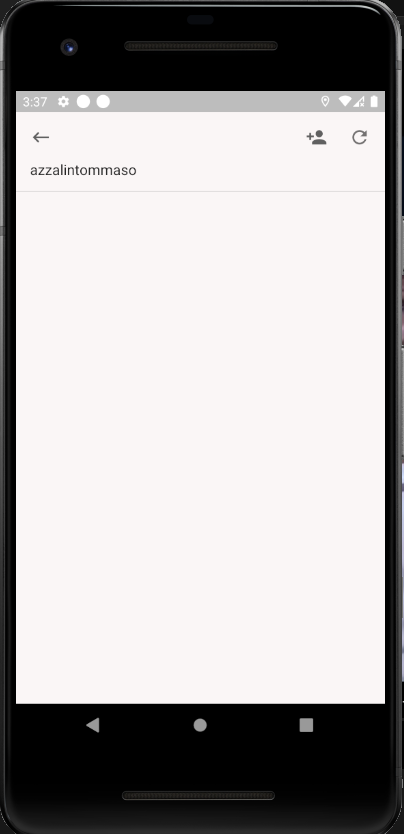
\includegraphics[width=0.4\textwidth]{images/app/friend/friend_overwiew}
    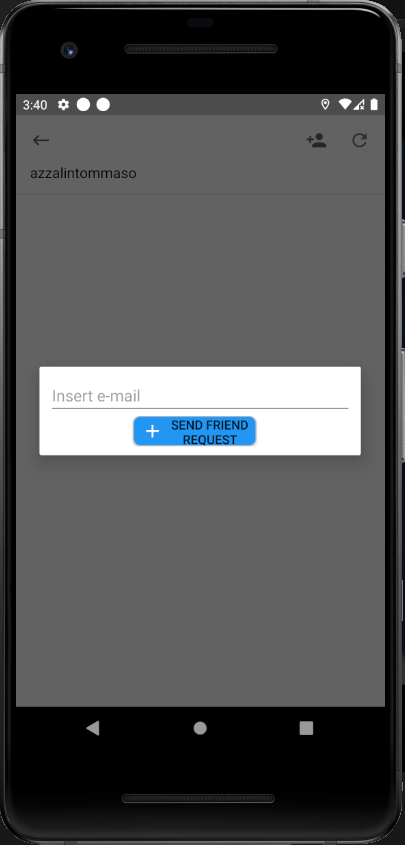
\includegraphics[width=0.4\textwidth]{images/app/friend/send_request}
    \caption{On the left, the \textbf{Friends} screen. On the right, the dialog to send a frienship request.}
\end{figure}

\noindent
When users receive a friend request they can either accept it or deny it. To do this, a dialog pops up after clicking on the notification and, when a user confirms it, the sender receive a notification.
An example is shown below.
\begin{figure}[H]
    \centering
    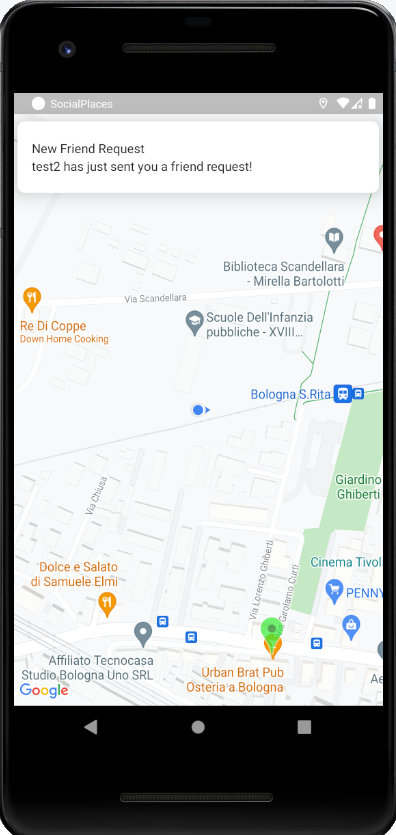
\includegraphics[width=0.3\textwidth]{images/app/notification/friend/friend_request_notification.png}
    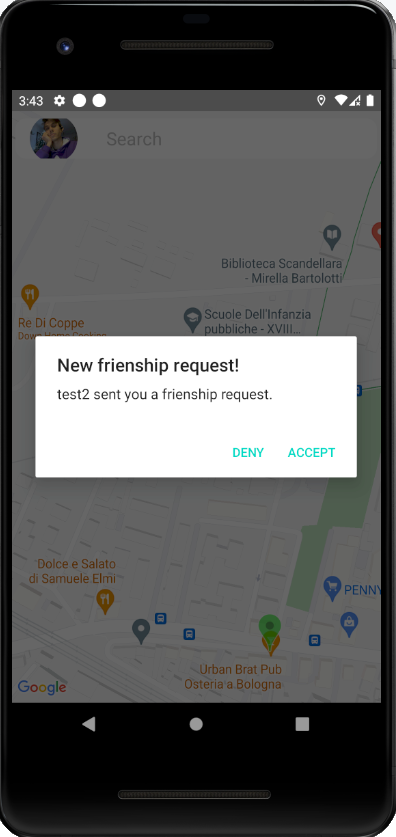
\includegraphics[width=0.3\textwidth]{images/app/notification/friend/dialog_friend_request.png}
    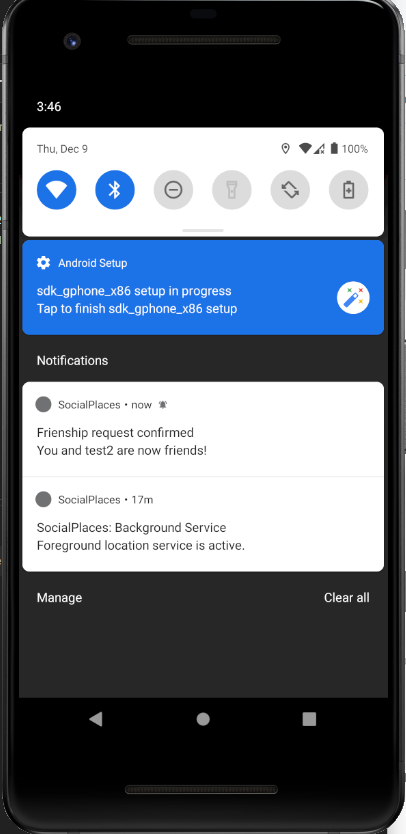
\includegraphics[width=0.31\textwidth]{images/app/notification/friend/confirmed_request.png}
    \caption{On the left, the notification of a friendship request. On the center, the dialog to accepty or deny a friendship request. On the right, the notification of a confirmed friendship request.}
\end{figure}
\noindent
Users can also see the public \textit{pois} of their friends and add them to their list, as shown in the pictures below:
\begin{figure}[H]
    \centering
    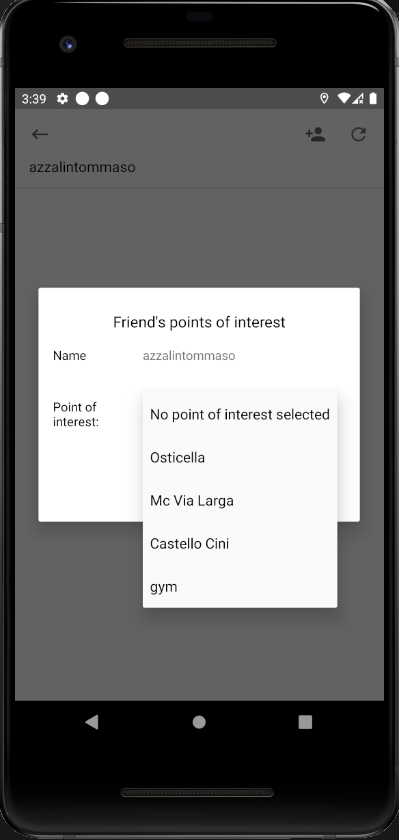
\includegraphics[width=0.4\textwidth]{images/app/friend/friend_poi}
    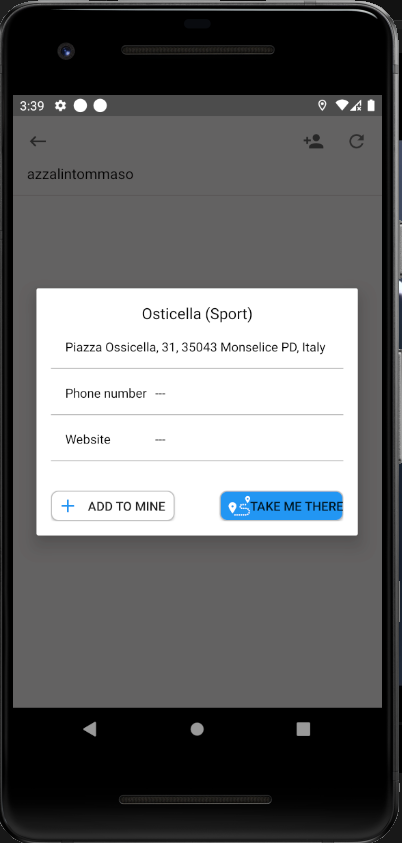
\includegraphics[width=0.4\textwidth]{images/app/friend/add_friend_poi}
    \caption{On the left, the list of public \textit{pois} of a user's friend. On the right, the dialog to add a poi to the user's personal \textit{pois} list.}
\end{figure}

\end{document}